\chapter[Password Personality]{Understanding Password Selection Through the Lens of Personality Traits}\label{chap:pws_and_personality}

%\section{Introduction}
% general introduction
% show that not *everyone* does the same
% selection is an individual task, not everyone selects passwords in the same way
Although there are certain patterns, password selection is a task that each individual handles in their own way. 
% even perception differs.
We have shown in chapter \ref{chap:pasdjo} that password strength is even subjectively \textit{evaluated} differently depending on certain characteristics. Again, while there was an overall tendency, we were not able to break down the strength ratings by individual differences: was there a special user group who performed better than others in the game? What characterizes this user group? Moreover, our previous chapter shed light on password policies in the wild. In a few notable cases, the rules were challenging and reject a substantial part of passwords. Users have developed strategies to cope with rejected passwords, but it would be interesting to know the exact factors that contribute to their behavior in these circumstances. Egelman and Peer make a strong argument that there is no ``average user'' so it is necessary to look at individual differences to understand user behavior \cite{Egelman2015AverageUser}. 

% personality traits in cybersecurity are a thing
Demographic background is one of the external factors that influences password selection \cite{Mazurek2013Measuring,  Violettas2014PasswordsAvoidGreece, Wang2015ChinesePWs}. Personality traits have been brought into the discussion to explain user preferences, actions, and behaviors in security questions \cite{Brown2004GeneratingPWs, Gross2016EffectCognitiveEffort, Shropshire2006PersonalityITSec, Zakaria2013DesigningEffectiveSecurityMessages}. Especially in research about phishing susceptibility we find evidence that personality traits have the potential to explain behavior \cite{Halevi2013PilotStudyPersonality,Halevi2015SpearPhishing,ParrishJr2009PersonalityPhishing,Uebelacker2014SocialEngineering}. 
% personality traits even matter for passwords
Empirical results from password studies have been discussed and explained with different personality traits, too \cite{Haque2014PsychometricsStrongPassword,Weirich2001PrettyGoodPersuasion}. It is a evident that a user's personality shines through, when they select a word based on personal preferences. 
% characterize personality in this realm
Petrie classified users in distinct password personalities: family-oriented, fans, fantasists, and cryptics\footnote{The original survey is not available online anymore. In a personal inquiry with Ms Petrie, she said that the original data is with the firm who commissioned the survey. The aggregated statistics are available at \url{http://passwordresearch.com/stats/statistic130.html}, \la{29.01.2018}}. A LastPass report more roughly divides password usage into two groups \cite{LastPass2016PersonalitiesGetUsHacked}: Type A users want to stay in control and are driven to act securely, so they developed an elaborate system that they perceive as suitable. Type B users do not believe that their accounts are valuable to attackers, so they do not prioritize security over usability. 
% this kind of categorization is nice, but too rough, maybe something more sound would solve the situation.
Those two taxonomies stem from analysis of user-selected passwords, i.e. a retrospective evaluation. However, predictive approaches are under-explored. For instance, if a user is generally an emotional person, does this impact their password selection strategies? If a user is diligent in real life, do they invest effort to diligently craft passwords, too? 
%``I can't remember passwords anyway'' could be attributed to a person who is less conscientious and/or less neurotic. 
%Are neurotic people more concerned about password strength, because they fear attacks more?

% that's what we do.
In a series of user studies we explored the associations between personality traits and passwords. If such associations exist, a new range of support systems opens that are tailored to a user's personality. Current one-fits-all approaches could be re-designed radically. The research was carried out in cooperation with three students. In each separate project we focused on a different stage of the password life-cycle. Timo Erdelt investigated personality as predictor for the usability of composition policies \cite{Erdelt2017BA}. Paul Huber explored correlations between strength perceptions and personality traits \cite{Huber2016BA}. Finally, Aline Neumann examined personality factors in password selection \cite{Neumann2017BA}. In total, 453 individuals participated in three separate online studies. In the following chapter, the projects are put into context and their findings are discussed on a bigger picture. 

\subsubsection*{Research Objectives}
Our primary goal was to find ways to predict password behavior from personality traits. At this point, the discourse about risky passwords included personality factors as explanatory variables. However, only few empirical studies had been carried out to challenge the assumptions. We aimed to provide such empirical data and a discussion of the implications on the design of password policies and password authentication systems. For instance, adjusting requirements of password policies depending on the user's personality promises to reduce frustration of password selection. Thus, our over-arching research question can be framed as ``\textit{Does personality influence user's mental models of password strength and selection strategies?}''.

%more related work: Groß \etal \cite{Gross2016CognitiveDepletion}
%
%Goals/motivation: 
%- some publications tried interpreted their findings as a consequence of different personality traits. first mentioned in \cite{Weirich2001PrettyGoodPersuasion} that personality could make a difference -- however, this had never been tried to empirically measure. 
%- explore differences in certain coping strategies (selection and reuse) through the lens of personality
%- find suitable ways to adjust password policies \cite{Seitz2017PersonalizingPasswordPolicies} - when users need to reset their password, after they had used the service for a while. 
%
%We posed the following research questions before we set out to conduct the study.\\
%\textbf{RQ1 - Psychological Factors} How much do psychological factors affect the perceived strength of passwords?\\
%\textbf{RQ2 - Big-Five vs GDMS} Are the Big-Five traits stronger or weaker predictors for strength perception than other psychological variables?\\
%\textbf{RQ3 - Portfolio Factors} Is the personal password portfolio associated with strength perception?

\section{Background and Related Work}
%We position our work in usable security and privacy, in particular password research. Moreover, we include psychological models to better understand users dealing with passwords. 
In this section we give a brief overview about the characteristics of strong passwords and how users go about creating them. Moreover, we portray projects in usable security and privacy research in which the users' psyche has been the focus. 
% secondary
%premise
%influencing 
%preconditions


%Moreover, since sophisticated attacks often start with checking for already known passwords, obtaining clear text data goes along with attackers improving their approach. A password that was strong before can quickly become very weak.  
%TODO eventuell noch das DING WANG paper und oder das Neural Network Ding vom Melicher zitieren.

%\subsection{Studies of Personality in Cyber Security}
\subsection{Password Selection Preconditions and Context Factors}
%TODO subconscious? 
%not exhaustive
% DEMOGRAPHICS
However, apart from such conscious behavior, there may be other preconditions that make some users pick stronger passwords than others. In a large field study, Mazurek et al. found that computer science and engineering students created passwords that were less guessable than those from business or politics students \cite{Mazurek2013Measuring}. Beyond demographic background, context factors like the emotional state during password selection have also been investigated. 
% EMOTIONS
Gulenko examined the effect of presenting positive textual messages and icons during password selection and found benefits for the adoption of passphrases \cite{Gulenko2014PasswordsEmotion}. In contrast, putting users in a state of cognitive distress or depletion made participants choose weaker passwords in a large lab study \cite{Gross2016EffectCognitiveEffort}. 
% PAST EXPERIENCES / BREACHES / ATTACKS
Social pressure as another type of psychological leverage was investigated by Egelman \etal \cite{Egelman2013DoesMyPasswordGoUpToEleven}. While they argue that account value plays a superior role for the effectiveness of password meters, others have shown that the \textit{design} of a password meter does have a measurable impact on the effort users put into creating a password \cite{Ur2012HowDoesYourPasswordMeasureUp}. In summary, the literature shows that password selection depends on context factors beyond education and experience. 
\subsection{Personality Factors in Cyber Security}
In our work, we are interested in context factors of password strength originating from psychological variables like personality. One of the most commonly used models to characterize personality are the Big-Five traits (B5), also known as the five-factor model. Costa and McCrae \cite{Costa1992NEO} refer to the personality traits as \textit{openness to experience}, \textit{conscientiousness}, \textit{extraversion}, \textit{agreeableness}, and \textit{neuroticism} (OCEAN). The traits can be described with these exemplary adjectives \cite{McCrae1987ValidationFFM}:\\
\textbf{Openness:} imaginative, creative, curious, independent, liberal\\
\textbf{Conscientiousness:} careful, reliable, ambitious, scrupulous, neat, punctual\\
\textbf{Extraversion:} sociable, talkative, passionate, warm\\
\textbf{Agreeableness:} selfless, helpful, forgiving, cheerful, humble\\
\textbf{Neuroticism:} worrying, emotional, insecure, impatient, vulnerable, subjective

Most frequently, the influence of these personality traits have been explored for privacy-concerns, where the openness trait was associated with privacy attitudes \cite{Egelman2015PredictingAttitudes,Minkus2014PersonalizationPrivacy}. Other inquiries have shown that personality traits like neuroticism \cite{Halevi2013PilotStudyPersonality} or openness \cite{Uebelacker2014SocialEngineering} might be associated with the response to phishing attacks. The likelihood of employees adhering to security policies is potentially influenced by the manifestation of agreeableness and conscientiousness \cite{Shropshire2006PersonalityITSec,Shropshire2015}. These investigations show that personality trait models are a considerable factor in security and privacy. Yet, our understanding of the influence of personality on password perception and consequently password selection is still low. Our work tries to improve our understanding about the origin of the differences in users' judgments of password strength. 
%is linked to these aspects, because passwords protect privacy of users and sensitive data of companies. %However, how password behaviors are formed and how much of the  is explained by psychological factors is still underexplored

%%%%%%%%%%%%%%%%%%%%%%%%%%%%%%%%%%%%%%%%%%%
%%%%
%%%%
%%%%			STUDY  1 ONE EINS
%%%%			POLICIES
%%%%
%%%%
%%%%%%%%%%%%%%%%%%%%%%%%%%%%%%%%%%%%%%%%%%%
\section{Study 1: Policies}
% general motivation - why do we investigate this?
We start out with the exploration of psychological factors for the design of password policies. We were motivated by the fact that at this point, policies are a one-fits-all solution that evidently does not work in the same ways for all users: Shay \etal observed that subjective usability ratings for policies differed among participants \cite{Shay2012CorrectHorseBatteryStaple, Shay2014CanLongPasswordsBeSecureAndUsable}. For instance, about 40\% of their participants found it difficult to create a password under a ``3class16'' policy, but another 40\% found it easy \cite{Shay2014CanLongPasswordsBeSecureAndUsable}. Following the general discourse and related results from privacy research, we hypothesized that an individual's personality might be responsible for their attitudes towards one policy or another. Therefore, our goal in this project was to explore such associations between personality traits and policy preference. 
%GOALS: explore associations between big-five traits and password selection under different policies, both on usability and security metrics. Investigate the effects of using a non-traditional password policy based on emojis. user preference for one policy or another. explorative study so no p-values.
\subsection{Method}
% general methodology
Our study was completely exploratory, because the literature did not allow us to derive narrow hypotheses. Since personality traits are nuanced, we opted for an online survey to collect a larger sample. Personality was assessed in the Five-Factor Model. We opted for the BFI-K construct by Rammstedt and John \cite{Rammstedt2005BFI}, because it is freely available in German. Moreover, with its 21 items, the time to fill out the questionnaire is kept reasonably low. 
Participants were asked to create several passwords in a row, i.e. the study followed a within-groups protocol. Here, we evaluated three different password policies: a traditional (3class12), an uncommon (2word12), and a novel policy (emoji12) that required the selection of at least one emoji through a graphical user interface (more on emojis in chapter \ref{chap:emojipasswords}). The reason for this choice was that the policies are different enough to serve as levels of the independent variable ``policy''. Participants assessed the ``difficulty to create'' a password for each policy. Moreover, we had them rank the policies by their personal preference, so the choice of 3class12, 2word12, and emoji12 would help them spot and judge the differences easily. 

\subsubsection{Structure and Tasks}
The study was divided into 3 overall parts. In the first part, participants were briefed about privacy details of the study and they provided demographic background information. Then they proceeded to the personality questionnaire before they were asked to perform three experimental tasks. Each consisted of creating a password and assessing the difficulty with agreement levels on the three items \textit{``It was difficult to create a password that meets the requirements''}, \textit{``I found the password requirements bothersome''}, and \textit{``It was easy to create a \textit{new} password''}. Agreement was measured on a five-point scale ranging from ``Strongly disagree'' to ``Strongly agree''. Inversely keying the items as well double encoding makes the data more robust against implausible responses. 

The order of the policies was counterbalanced to mitigate order effects, we recorded the order as a control variable. We chose an online-banking scenario for all three selections. The first prompt was to create a password to protect an online banking account. Secondly, participants were told that someone had gained access to their account and the bank locked them out. As a security precaution, they had to reset their first password. The last task description explained that their password had expired after one year and they need to reset it again. This storyline was designed to fulfill the \textit{realistic threat} principle proposed by Krol \etal (see Section \ref{sec:rw:principles-experiments}) \cite{Krol2016ExperimentDesign}. 

We used SosciSurvey, a standard survey tool, to collect the responses. The dynamic parts involving password selection were embedded in iframes. To match the data from the survey tool and the iframe we used URL query parameters containing the response ID. We asked participants to switch to a desktop browser to avoid styling glitches and unexpected behavior from the prototypes. %Auto-complete was prevented in any case

\subsubsection{Recruiting and Demographic Background}
We recruited participants through posts on social networks and by sending out the invitation link in a university-wide newsletter (more than 5000 recipients). To incentivize participation, we announced a raffle of five shopping vouchers with a value of 20€ each. At this point, 222 people had started participation. After drop-out and plausibility checks, the remaining sample size was $N=164$. As expected, the age distribution was narrow: our sample consisted mostly of students in their mid-twenties \average 24.7 (SD=5.5). 79 respondents were female, 83 male, and 2 preferred not to answer. In the background screener, 65 people (40\%) indicated to possess formal training in computer science or information technology. We also requested self-reported assessments on password behaviors. Here we found that 40\% reuse passwords without modification, 32\% reuse them with modifications or with a mnemnoic technique. 17\% often create new passwords. In terms of management strategy, the majority (53\%) tries to memorize passwords. 11\% use a password manager or generator. Written cues served as aid for 10\% of respondents, and 16\% write passwords down on analog media, while 21\% use electronic files. Interestingly, the distribution of coping strategies is very close to survey findings gathered with more diverse samples \cite{CSID2012PasswordHabits}. Hence, we believe to have caught a representative snapshot of password behavior.

\subsubsection{Statistical Analyses}
For statistical analyses, we consulted the StabLab\footurl{http://www.stablab.stat.uni-muenchen.de/}{30.01.2018} to identify suitable methods. After a revision of the collected data and the necessary assumption checks, the associations were explored with additive models (AM). Their advantage over linear regression is more flexible for non-linear associations \footurl{https://en.wikipedia.org/wiki/Additive_model}{30.01.2018}. The \textit{mgcv} package for R was used to calculate the models.

Scores on the Big-Five sub-dimensions served as independent variables, i.e. the predictors in the regression models. \textit{Openness} is coded with five items, while the remaining four dimensions were assessed with four items. The agreement levels for each item were mapped to numeric values from 1 to 5. The score on a sub-dimension is the sum of agreement levels. To better estimate effect sizes, we control for gender, age and IT proficiency in the models. 
\subsubsection{Method limitations}
The method, albeit carefully executed, faces a few limitations regarding the interpretability. First, the sample was fairly homogeneous, because participants were mostly between 20 and 28 years old and have an academic background. However, personality traits are not age dependent \ar?. Our study was strongly focused on individual preferences and usability perceptions of different policies, so only a within-groups design was feasible. However, in real-life password selection, users rarely select three passwords in a row. The choice of our storyline still makes confident about the ecological validity \cite{Fahl2013EcologicalValidityPasswordStudy}. The repeated measures design did not allow us to measure the policies' influence on password memorability, which we have to postpone to another study. At this stage, the preference was more valuable for our exploration than memorability effects. Besides, we briefed participants to fill out the survey on a desktop PC or a similar device. We cannot guarantee that all participants followed this instruction, which might have had an effect on their password selection \cite{Melicher2016UsabilityMobileTextPasswords}. 

Finally, we unfortunately made a mistake in the deployment of the emoji-based policy. Instead of 12 characters, it required participants to select 16 characters beside the emoji. We realized this fact by looking at descriptive statistics during the course of the study, because the policy performed significantly worse than the other two. We re-deployed the emoji-based policy immediately after we had realized the error. Consequently, we had to remove the data for the creation difficulty and ranking in cases 1-61, reducing the overall sample size to 103. Nonetheless, the sample size is sufficiently large to investigate medium to strong effects. 

%- we started out with emoji16, but made the switch to emoji12 (after 43 participants), because emoji16 received the most negative feedback, but it was mostly due to the length. data removed for ranking (1-61) and difficulty to create (1-43). 

\subsection{Results}


medium associations between extraversion, agreeableness, and neuroticism (basically the other three dimensions that were not useful before), but control variables are associated to a larger degree.

emoji policy similar results as traditional policies, i.e. it is wortwhile to experiment with it

\paragraph{Descriptives and Hypothesis Tests}
creation difficulty: Repeated measures linear mix model ANOVA. random intercept to account for the fact that people generally rate policy usability low. baseline (any could be chosen) emoji 12.

emoji \average 7.89 (in [3;15] range), 2word12 + 0.12, 3class12 - 0.70 (easier)
serial positioning effects do make a difference, but it also appears trivial in the overall sample.
summary: no big difference between policies and ranking. (this is what makes the remainder more exciting, because a closer look at the data brings out how the numbers come to be)


\paragraph{Creation Difficulty}
% gender
Female participants reported more difficulties for emoji12 ($\beta=0.91$) and 2word12 ($\beta=1.35$). 
for 3class12 correlation was smaller ($\beta=-0.46$) and pointed in the opposite direction.
% it background
IT background revealed interesting effects too: emoji12 ($\beta=-0.10$) trivial, 3class12 ($\beta=0.21$) weak, 2word12 ($\beta=0.61$) medium. it looks as though people with higher IT knowledge struggle with a word-based policy, potentially because it is much less common in the wild. 
% order of the policy
If you factor in the order of the policy, the results look clearer. if emoji12 and 3class12 were shown in position 2, creation was more reported to be more difficult emoij12-2 ($\beta=0.52$), 3class12-2 ($\beta=1.19$) 
% age
we observed non-linear associations between age and creation difficulty, but the small age range forbids us to make conclusive inferences from our data.

%emoji personality
mostly non-linear associations for the emoij12 policy
neuroticism weak linear association emoji12 ($\beta=-0.22$), i.e. it was slightly easier for people with higher neuroticism scores (this is a great result, albeit weak. neurotic people are by defintion more \textit{emotional}, and emojis seem to cater to this trait.)
agreeableness weak non linear, and interesting curve (up and down) for emoji12
openness weak non linear, but too little data to conclusively decide. 
% 2word12 personality
effects not as clear as for the emoji policy. highly open people report slightly less difficulty to create a 2word12 password.

% 3class12
linear associations are negligible for extraversion, conscientiousness, and neuroticism. 
non-linear associations for agreeableness and openness. at value around 15 (from 20) the difficulty seems to increase (hard to interpret this finding). People with agreeableness scores of 18 and greater find it more difficult to create a 3class12 password by up to 1.5 points. Openness is inversely correlated here. the more open the participant was, the more likely they found it easy to create a 3class12 password. 


\paragraph{Ranking}
logistic additive regression %https://web.stanford.edu/~hastie/Papers/AdditiveLogisticRegression/alr.pdf
did policy X land on top spot ? yes = 1, no = 1. thus, no encompasses the two other options.
Logit model. see timo's work to better understand what's going on. 

\begin{table}
	\centering
	\caption{\label{tab:pws_pers:distribution-binary-ranks} Distribution of binary rankings of the three available policies. Evidently, 3class12 was ranked best in most cases. }
	\begin{tabular}{llll}
		~ 			& emoji12	& 2word12 	& 3class12 \\ \hline\hline
		1st rank	& 18		& 12		& 67 \\
		other rank 	& 80 		& 85 		& 31 \\ \hline
		n			& 98		& 98		& 98		 
	\end{tabular}
\end{table}


% predictors: demography and structure
strong effects. the probability of a non-IT person putting emoji12 at the top is $exp(\beta–{IT-0}=9.87)$, so around ten times higher. only one IT-person ranked emoji12 first. (this fits to the finding that non-IT people found it easier to create an emoji12 password).
% order of policies 
the order in which policies were displayed also produced a notable effect. If emoji12 is shown in 2nd $exp(\beta–{emoji-pos2}=0.27)$ or 3rd position $exp(\beta–{emoij-pos3}=0.76)$, the likelihood to rate it the best policy slightly decreases. Other positionings, as well as age-related preferences, were inconclusive.

% personality
generally weak associations.
extraversion, weak linear effect regarding 2word12. likelihood to put 2word12 first decreases with higher extraversion scores $exp(\beta–{E-1}=0.82)$. for agreeableness both linear and non-linear effects are visible; higher scores increase chances to vote emoji12 first $exp(\beta–{A-1}=1.28)$. openness or conscientiousness have negligible, random associations. for neuroticism we lack data in edge cases (low or high trait scores) to draw conclusions. %there are more results in the BA, but I do not really see the point of reporting all the details of inconclusive results


\paragraph{Password selection}

\todo{create a emoiji selection histogram}. In essence, some emoji were strongly preferred, e.g. the red heart and the ``pouting face''. analyze: what were the usability ratings/rankings of those who picked the heart vs. the pouting face, i.e. are emojis with a positive connotation used by people who are happy that they can select an emoji password? I guess there are significant effects here. 

\subsection{Lessons Learned}
It could have been useful to include a recall test à la ``which passwords do you still remember after filling out the personality questionnaire?'' 

\subsection{Discussion}
%TODO re-read the discussion section, because the findings are a bit higher level and more understandable
Most interesting finding: Non-IT people significantly less likely to put emoji policy first. s

emoji (negatively) associated with emotional stability, i.e. less stable people who are more emotional in either direction were more positive towards emojis.

non linear associations probably explicable by other variables, e.g. intercorrelation -- 
\todo{discuss the personality traits and associations, try to explain them.}

demographics play a role - (careful now, cowboy): policies could be tailored to gender. but i'm kind of reluctant to put this argument forward. at least IT background could be considered a factor for the policy. a personalized policy would make it more difficult for horizontal attacks because the policy is unpredictable.

mutually exclusive effects for ranking are clear because of the binary nature.

wild idea: if positioning influences the favorability of policies, one could leverage this. like anchoring and decoy (chose your own policy of the three). commitment and consistency as well (commit to your policy, create a strong password to be consistent with your commitment.)

%%%%%%%%%%%%%%%%%%%%%%%%%%%%%%%%%%%%%%%%%%%
%%%%
%%%%
%%%%			STUDY  2 TWO ZWEI
%%%%			PERCEPTION
%%%%
%%%%
%%%%%%%%%%%%%%%%%%%%%%%%%%%%%%%%%%%%%%%%%%%
\section{Study 2: Strength Perceptions}
With an observational online study, we explored the associations between psychological variables and password strength perception. As outlined in Chapter \ref{chap:pasdjo}, we regard the perception of strength as an implicit driver for behavior, which is more difficult to observe. Hence, we explored associations between subjective password strength ratings and scores on well-established psychometric scales. 
%task description
The task resembled the PASDJO game: participants were shown a password, and they had to rate it on a seven-point scale. We chose seven point scales to make the approach more comparable to Ur \etal \cite{Ur2016PerceptionsPassword}. Moreover, we gave participants two passwords, and they had to decide which one was stronger. 

%pre-registration
Before we ran the study, we pre-registered the experiment with the open-science framework (OSF)\footnote{\url{https://osf.io/}, last accessed 11.09.2016} and planned to conduct all analyses as predicted to mitigate confirmation bias. However, the envisioned statistical  tests were not always applicable, which forced us to consider more appropriate methods and move away from the pre-registration. Since we consider our research efforts mostly exploratory, we approached the study without specific hypotheses regarding the influence of certain personality traits on the perception of password strength.

\subsection{Structure}
% First Part: DEMOGRAPHICS
The study was divided into six parts. Two parts were standard psychometric tests. We describe all parts, to give the reader the full picture about the participants' tasks. However, we have to omit a few less important results for the sake of clarity. After a brief introduction where the participants were informed about the background of the study, the first step was to provide basic demographic information regarding gender, age, educational and professional background. %This information is important for the ratings on the password scales, because advanced knowledge in IT(-security) may lead to a different rating than the general audience. 

% Second Part: META STATISTICS / CREATION
\paragraph{Meta Password} The second part elicited characteristics about the passwords that our participants used on real online accounts. Here, we asked about typical password attributes, like LUDS (lower-, uppercase, digits, symbols), length and the inclusion of dictionary words. The collection of such password descriptions is an ethically reasonable way to study actual behavior that does not directly involve creating and disclosing an entire password \cite{VonZezschwitz2013SurvivalShortest}. Participants could select from a list of accounts that they used on a regular basis, e.g. Facebook, YouTube, Netflix, Google. If they did not have any of the selectable accounts they could provide another. We call the description of a participant's password on any of these sites ``\textit{meta password}'' in the remainder of the chapter. We included this part in the survey to explore additional covariates for strength perception.
%TODO entscheiden ob das reinkommt Additionally we had them create a password which they would rate as sufficient to protect such an online account and that is memorable. We asked not to enter a password that they were currently using. At the end of the study, we again inquired after the fictional password to measure short-term memorability. 

%%% TABLE: PASSWORDS
\begin{table}[htbp]
  \centering
  \caption{Set of passwords that we divided into different length and strength categories (as measured with zxcvbn). Features: U = uppercase, D = digits, S = symbols}
 % \small
    \begin{tabular}{lllcccr}
    \multicolumn{1}{c}{\multirow{2}[1]{*}{Password}} & \multicolumn{2}{c}{Categories} & \multicolumn{3}{c}{\multirow{2}[1]{*}{Features}} & \multicolumn{1}{c}{guesses} \\
      & Length & Strength & \multicolumn{3}{c}{} & \multicolumn{1}{c}{(log10)} \\
    \midrule
    hagrqqqqthhbbe & Long & Strong & \multicolumn{3}{c}{-} & 12.48 \\
    etuhcarap & Short & Weak & \multicolumn{3}{c}{-} & 4 \\
    AbWxCdYz & Short & Medium & \multicolumn{3}{c}{U} & 8 \\
    1qaz2wsx3edc & Long & Weak & \multicolumn{3}{c}{D} & 3 \\
    a6a4ba8a & Short & Medium & \multicolumn{3}{c}{D} & 8 \\
    ieatkale88 & Short & Medium & \multicolumn{3}{c}{D} & 10 \\
    thedzfhg123 & Short & Medium & \multicolumn{3}{c}{D} & 10 \\
    11Nd1sPPut8ble99 & Long & Strong & \multicolumn{3}{c}{U,D} & 16 \\
    bicycles-peaches-cold & Long & Strong & \multicolumn{3}{c}{S} & 13.69 \\
    AatIcs,ijayl-t & Long & Strong & \multicolumn{3}{c}{U,S} & 13.95 \\
    p@ssw0rd & Short & Weak & \multicolumn{3}{c}{D,S} & 0.95 \\
    ocean4 Size !beer Car & Long & Strong & \multicolumn{3}{c}{U,D,S} & 20.39 \\
    F@m1Ly07\% & Short & Medium & \multicolumn{3}{c}{U,D,S} & 6.88 \\
    \bottomrule
    \end{tabular}%

  \label{tab:password-list}%
  
\end{table}%

% Third Part:  RATING
\paragraph{Standalone Strength Rating} In the third part of the study, the \textit{rating part}, the participants assessed the strength of one password at a time in random order, similar to playing PASDJO. The passwords had to be rated on 7-point scales ranging from \textit{1 = very weak} to \textit{7 = very strong}. We picked a set that was comparable to related work \cite{Ur2016PerceptionsPassword} and that we carefully designed around certain attributes. Table \ref{tab:password-list} shows the selected set of passwords and their features. The ``length'' category distinguishes between short passwords with nine characters or less and long passwords with ten characters or more. The distinction is inspired by real-world policies that most commonly require up to nine characters (see Chapter \ref{chap:policies_reuse}). The ``strength'' category groups passwords on three levels by their guess number as determined by zxcvbn. Weak passwords require less than $10^{6}$ guessing attempts, strong passwords at least $10^{12}$ guesses, and medium passwords anything in between. This classification is in concordance with related work \cite{Florencio2014AdministratorsGuide, Wheeler2016zxcvbn} . To fully counterbalance all category combinations, one would require 120 items, which we could not implement for the sake of brevity. Hence, we kept the number of items small to mitigate fatigue during the study sessions. In the chosen set of 13 passwords, there were at least three items for each distinct category, i.e. three short, long, weak and strong passwords, and at least three passwords pertaining to different LUDS policies (lowercase, uppercase, digits and symbols).

% Fourth Part: COMPARISON
\paragraph{Comparison} Following a similar procedure as Ur et al. \cite{Ur2016PerceptionsPassword}, participants moved on to compare the strength of passwords pairs (\textit{comparsion part}). The 7-point scale ranged from ``<left password> is much stronger'' to ``<right password> is much stronger''. The pairs were constructed such that the passwords differed, e.g., in the existence and positions of digits and uppercase letters. Figure \ref{fig:comparisontask} illustrates our scoring schema. 

\begin{figure}
	\centering
	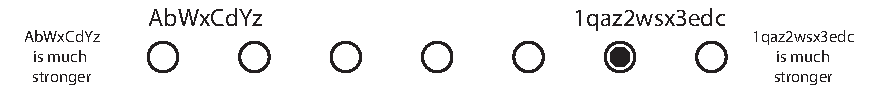
\includegraphics[width=\linewidth]{figures/comparisontask}
	\caption{\label{fig:comparisontask} Simplified item of the comparison task. The passwords differ in length, strength, and the usage of uppercase letters and digits. Here would have scored the importance of length and digits with +2 while the importance of strength and uppercase letters was scored with -2.}
\end{figure}

If the passwords measurably differ in strength as in Figure \ref{fig:comparisontask}, the ratings show if the participants' perceptions match reality. In total, ten comparisons had to be made in random order, in which we permuted the combinations. For this task, we also added an attention check where the passwords on both sides of the scale matched, allowing us to exclude responses where the answer differed from ``both passwords are equally strong''. 

\paragraph{SeBIS} Next, we requested self-assessment about security-related behavior using the Security Behavior Intentions Scale (SeBIS) \cite{Egelman2015SeBIS}. This scale comprises the dimensions \textit{securement}, \textit{passwords}, \textit{awareness}, and \textit{updating}. For each dimension, a score is calculated with four items totaling up to 16 additional items in our study. However, in discussions after the experiment we received hints that it would have been better to include a gap of a couple of days before collecting the SeBIS data to ensure its validity. Since we failed to take this into account beforehand, we do not report the results further, but it is important to mention that the questionnaire included those 16 items. 
%The items are phrased as statements to which respondents can indicate how often they show a certain type of security-related behavior. The scale ranges from \textit{1 = never} to \textit{5 = always}. The \textit{password} dimension measures general attitude towards passwords, which we can utilize to inform our interpretation later.

\paragraph{Big Five} The study concluded with two psychometric tests. In the \textit{Big-Five part}, we utilized a set of 50-items from the International Personality Item Pool (IPIP), which is a representation of Costa and McCrae's NEO-PI-R domains \citep{Costa1992NEO}\footnote{All items of the personality test can be found here: \url{http://ipip.ori.org/newNEODomainsKey.htm}, psychometric properties: \url{http://ipip.ori.org/newNEO_DomainsTable.htm}}. In this personality test, participants rate how accurately a certain statement portraying a certain personality characteristic describes themselves. Each item is a 5-point scale with the labels \textit{very inaccurate, moderately inaccurate, neither accurate nor inaccurate, moderately accurate, very accurate}. Every personality trait is tested with five positively and five negatively keyed items. It was shown that the 50-item version of the test shows high correlation with more exhaustive tests ($r > 0.75$ in all dimensions) and is thus a sufficiently reliable test. We randomized the order of the items.

\paragraph{GDMS} Egelman and Peer found that the general decision-making style had higher predictive power than the Big-Five traits for privacy-related behavior \cite{Egelman2015AverageUser}. Thus, we wanted to test the feasibility of both psychometric tests and finished the study with the \textit{GDMS part}. This scale uses 25 positively keyed items to measure the five decision-making styles \textit{rational}, \textit{intuitive}, \textit{dependent}, \textit{avoidant} and \textit{spontaneous}. 



\subsection{Quantitative Analysis}
Since at least three passwords showed a certain characteristic, e.g. uppercase letters, we averaged the ratings for them accordingly and used them as dependent variables. Moreover, in the psychometric tests we accounted for negatively keyed items, i.e. those items that were phrased with negations like \textit{``I don't talk a lot''}. We inverted the ratings where necessary and afterwards calculated the sum of agreement levels for each dimension (\textit{trait score}). 

%cleaning the data
As in Section \ref{sec:personality:study-1}, we repeatedly fit a \gls{GAM} to our data, i.e. a more flexible and interpretable form of regression\footurl{https://multithreaded.stitchfix.com/assets/files/gam.pdf}{06.02.2018}. 
%DV
Subjective password strength assessments, respectively comparisons, serve as dependent/response variables. We calculate one score per participant and password category by adding up the corresponding ratings. For instance, if they rated all eight passwords containing digits with seven points, their score for ``G\_Digits'' (\textbf{G}roup of passwords with digits) is 56. We average participants' ratings for models that require means instead of total scores. 
%Only to compare the means in each password category, we average the ratings. 

%IV
Psychometric scores on all several sub-dimensions served as independent variables (covariates). We always control the regression models for gender, technical background and age to contrast effects. Wherever possible, we model covariates as linear, if the GAM indicates that smoothing is unnecessary. For this data-set, we also conducted principal component analysis followed by factor analysis. The resulting factors are then used to fit additional models for comparison. This allows us to evaluate the suitability of the Big Five inventory for our exploration.
%Since some \gls{GAM} smooth terms might make models worse, we use automatic penalization to basically remove them from the model\footurl{https://www.rdocumentation.org/packages/mgcv/versions/1.8-23/topics/gam.selection}{06.02.2018}. 

%We check for collinearity using variance inflation factors (VIF) and only retain factors with VIFs close to 1 \cite[p. 217]{Weisberg2005applied}. 
%Finally, we perform Durbin-Watson tests to rule out auto-correlation effects (target value $d=2$). While p-values do not add much to the interpretability of the findings, we report them for the sake of completeness.  
%TODO Quelle!
%Our level for statistical significance is $\alpha = 0.05$, unless Bonferroni correction requires a lower value. 

%When we report the results of linear regression models, we only do so for the models with the highest adjusted $R^2$ value, i.e. the model where the number of predictors leads to the best model-fit explaining the variance in the dependent variable. The values in Tables \ref{tbl:personalpw_regression} through \ref{tab:Comparison-Regression} are the \textbf{standardized beta} correlations, i.e. they are unit-less and lie between -1 and +1. 

\subsection{Qualitative Analysis}
To better understand the reasoning behind the ratings and comparisons, we also inquired how the respondents approached the rating task. They could enter free-text answers after all ratings were done. The answers were then coded independently by two members of the team. The first coding step was to find categories and propose the code book. Afterwards, the proposed codes were handed over to the second coder, who sorted answers into the categories and amended new ones where necessary. Interrater agreement between the two coders was satisfactory (78\%, Krippendorff's $\alpha = 0.55$) and the final the code book could be created after discussing the discrepancies. We report how many participants mentioned a particular theme in their response regarding their rating strategies.


\subsection{Recruitment}
We utilized the online research platform Prolific\footnote{\url{https://prolific.ac}, accessed 01.09.2016} to administer our survey. Participants received \$2.65 upon successful completion, which took 20 minutes in average. This compensation level is suggested as part of the ethical reward guidelines on the platform. Only an English-speaking audience was eligible to participate. From the 178 people who started the survey, 104 finished it. To prevent low quality answers, we introduced an attention check during the comparison part of the experiment.  



\subsection{Ethical Considerations}
There is no institutional review board for this kind of studies at our institution. However, we designed the questionnaire to respect the participants' privacy and did our best to minimize the level of disclosure of sensitive data. The metrics we collected to characterize the participants' passwords are most likely insufficient to reconstruct the passwords in a straightforward way and can thus be considered ethically acceptable. 


\subsection{Limitations}
%It is good to discuss the limitations before the results. Thus, the reader can bear them in mind when they are reading on. 

Like most studies involving personality assessment, the result is only a rough model of a person's personality and does not include all facets. We chose a test with 50 items to assess the Big-Five traits. While such psychometric tests exist with item counts between 10 \cite{Gosling2003TIPI} and 240 items \cite{Costa1992NEO}, the 50-item version has high internal reliability and does not fatigue the respondents as much as more exhaustive tests. Additionally, with a sample size of 100 participants, power-analysis tells us, that only strong and medium interactions are likely to be found for with our regression models (cf. \cite{Shevlin1998SampleSize} or \cite[p. 223]{Field2005DiscoveringStatistics}). At this stage of the exploration, however, this is what we aimed for. If we do find effects with such a small sample, then they must be large enough to justify follow-up investigations with larger samples. Moreover, statistical analyses can be done very differently. We traded off model complexity and interpretability to draw first conclusions. Thus, the reported associations can never be seen \textbf{causal effects}, because we would have to use different experimental setups, and carry out the experiments many times on larger samples. In the scope of our personality studies, we therefore provide pointers and possible explanations, but do not claim that the results are highly generalizable. This is especially important, because the sample stems from a technically savvy audience. Users registering for tools like Prolific or Amazon Mechanical Turk may also have stronger financial motivation to do so than the rest of the population \cite{Ross2010WhoAreTurkers}. 

Furthermore, the methodology relies on self-assessment and honest answers, which are difficult to control. We introduced an attention check to mitigate the problem, by asking people to compare two identical passwords. For the meta-password, we do not know whether it was created on a mobile or desktop device. Passwords created on mobiles are usually less complex than those created on desktops \cite{Melicher2016UsabilityMobileTextPasswords, VonZezschwitz2014HoneyIShrunkTheKeys}. 

Finally, the study set-up and procedure may also influence the interpretability of the outcome. We decided not to randomize the order of the question blocks to maintain full control over the general procedure. When we measure dependent variables, the order of questions is still randomized in the question groups. This way, the potential fatigue effects are the same for all participants at the different stages, while the important questions are in random order. Moreover, the items for password pairs were not fully counterbalanced on all levels to prevent fatigue when answering the entire questionnaire. A more exhaustive set of tested passwords would increase the generalizability. 



%%%%%%%%%%%%%%%%%%%%%%%%%%%%%%%%%%%%%%%%%%%
%%%%
%%%%
%%%%			RESULTS 
%%%%
%%%%
%%%%%%%%%%%%%%%%%%%%%%%%%%%%%%%%%%%%%%%%%%%
\subsection{Results}
In this section, we first describe the participants and meta password characteristics before we proceed to the regression analyses. Since we created plenty of regression models, we only report those who showed notable associations -- mostly for ``Overall'' and ``Digits'' in the rating part, and ``Symbols'' and ``Digits'' in the comparison part. We omit results from other psychometric measures (GDMS, SeBIS) for the sake of stringency. The final part of this section shows qualitative findings and a brief synthesis of the results. 

\subsubsection{Participants}
We collected 104 complete samples. We had to remove three samples from respondents who failed the attention check. Another response was removed because all responses on point scales were answered with the same value. This procedure is proposed by the IPIP project\footnote{\url{http://ipip.ori.org/newValidity.htm} accessed 02.09.2016}. The resulting total N = 100 was divided into 42 female and 58 male participants. Their average age was 28 years ($Standard Deviation~(SD) = 9,~Minimum = 16,~Maximum = 61,~Median~(Md) = 26$). 44 responses came from students. The education level was high with 59 participants reportedly having a bachelor's (44) or master's (15) degree. 29 participants claimed to have a computer science or IT-related background. In summary, our sample stems from a young, educated and fairly technically savvy population. This convenience sample is not ideal, but we hope to deal with this skew by including demographics as predictors in the regression models.

\subsubsection{Ratings Descriptives}
On average, the respondents correctly identified weak, medium and strong passwords in the rating task, i.e. their perception matched reality. The average subjective scores were $M=3.60~(SD=1.07)$ for weak, $M=4.25~(SD=0.95)$ for medium and $M=4.71~(SD=0.90)$ for strong passwords. A Friedman rank test showed that these ratings differed significantly ($F(2)=59.91,~p < 0.001$). Figure \ref{fig:personality:study2:average-rating-boxplot} shows all averages per group.

\begin{figure}[htbp]
	\centering
	\includegraphics[width=\linewidth]{personality/avearge-rating-boxplot}
	\caption{\label{fig:personality:study2:average-rating-boxplot}}
\end{figure}

%%%%%% TABLE 
%\begin{table*}%[h!tbp]
  \small
  \centering
  \caption{Regression analysis for password ratings in different categories as dependent variables and psychometrics as independent variables variables. Demographic data serves as control variables. Numbers in bold indicate statistical significance ($p<0.05$). The Big-Five factors had higher predictive value and than the GMDS factors.}
    \resizebox{\linewidth}{!}
{
\begin{tabular}{rl|r|rr|rrr|rrr}
    \multicolumn{2}{l|}{Predictor} & \multicolumn{1}{l|}{Overall} & \multicolumn{1}{l}{Short} & \multicolumn{1}{l|}{Long} & \multicolumn{1}{l}{Weak} & \multicolumn{1}{l}{Medium} & \multicolumn{1}{l|}{Strong} & \multicolumn{1}{l}{Symbols} & \multicolumn{1}{l}{Digits} & \multicolumn{1}{l}{Uppercase} \\
\cmidrule{3-11}    \rowcolor[rgb]{ .718,  .871,  .91} \multicolumn{1}{l}{Big Five} & Neuroticism & \cellcolor[rgb]{ 1,  1,  1}  & \cellcolor[rgb]{ .949,  .91,  .518} 0.15 & \cellcolor[rgb]{ .949,  .91,  .518} 0.15 & \cellcolor[rgb]{ .969,  .914,  .518} 0.14 & \cellcolor[rgb]{ 1,  1,  1}  & \cellcolor[rgb]{ .98,  .627,  .459} -0.15 & \cellcolor[rgb]{ 1,  1,  1}  & \cellcolor[rgb]{ 1,  1,  1}  & \cellcolor[rgb]{ 1,  1,  1}  \\
    \rowcolor[rgb]{ .718,  .871,  .91}   & Openness & \cellcolor[rgb]{ .976,  .518,  .439} \textbf{-0.25} & \cellcolor[rgb]{ .976,  .541,  .443} \textbf{-0.23} & \cellcolor[rgb]{ .98,  .573,  .447} \textbf{-0.2} & \cellcolor[rgb]{ .976,  .498,  .435} \textbf{-0.27} & \cellcolor[rgb]{ .98,  .616,  .459} -0.16 & \cellcolor[rgb]{ .98,  .604,  .455} -0.17 & \cellcolor[rgb]{ .984,  .647,  .463} -0.13 & \cellcolor[rgb]{ .976,  .541,  .443} \textbf{-0.23} & \cellcolor[rgb]{ .984,  .639,  .463} -0.14 \\
    \rowcolor[rgb]{ .718,  .871,  .91}   & Agreeableness & \cellcolor[rgb]{ .898,  .894,  .514} 0.18 & \cellcolor[rgb]{ .949,  .91,  .518} 0.15 & \cellcolor[rgb]{ .898,  .894,  .514} 0.18 & \cellcolor[rgb]{ .898,  .894,  .514} 0.18 & \cellcolor[rgb]{ 1,  1,  1}  & \cellcolor[rgb]{ .969,  .914,  .518} 0.14 & \cellcolor[rgb]{ .984,  .918,  .518} 0.13 & \cellcolor[rgb]{ .996,  .91,  .514} 0.11 & \cellcolor[rgb]{ 1,  1,  1}  \\
    \rowcolor[rgb]{ .988,  .835,  .706} \multicolumn{1}{l}{GDMS} & Rational & \cellcolor[rgb]{ 1,  1,  1}  & \cellcolor[rgb]{ 1,  1,  1}  & \cellcolor[rgb]{ 1,  1,  1}  & \cellcolor[rgb]{ 1,  1,  1}  & \cellcolor[rgb]{ 1,  1,  1}  & \cellcolor[rgb]{ 1,  1,  1}  & \cellcolor[rgb]{ 1,  1,  1}  & \cellcolor[rgb]{ 1,  1,  1}  & \cellcolor[rgb]{ .984,  .918,  .518} 0.13 \\
    \rowcolor[rgb]{ .988,  .835,  .706}   & Intuitive & \cellcolor[rgb]{ 1,  1,  1}  & \cellcolor[rgb]{ 1,  1,  1}  & \cellcolor[rgb]{ 1,  1,  1}  & \cellcolor[rgb]{ 1,  1,  1}  & \cellcolor[rgb]{ 1,  1,  1}  & \cellcolor[rgb]{ 1,  1,  1}  & \cellcolor[rgb]{ 1,  1,  1}  & \cellcolor[rgb]{ 1,  1,  1}  & \cellcolor[rgb]{ .996,  .898,  .51} 0.1 \\
    \rowcolor[rgb]{ .988,  .835,  .706}   & Avoidant & \cellcolor[rgb]{ 1,  1,  1}  & \cellcolor[rgb]{ 1,  1,  1}  & \cellcolor[rgb]{ 1,  1,  1}  & \cellcolor[rgb]{ .984,  .639,  .463} -0.14 & \cellcolor[rgb]{ 1,  1,  1}  & \cellcolor[rgb]{ 1,  1,  1}  & \cellcolor[rgb]{ .984,  .647,  .463} -0.13 & \cellcolor[rgb]{ 1,  1,  1}  & \cellcolor[rgb]{ 1,  1,  1}  \\
    \rowcolor[rgb]{ .988,  .835,  .706}   & Spontaneous & \cellcolor[rgb]{ 1,  1,  1}  & \cellcolor[rgb]{ 1,  1,  1}  & \cellcolor[rgb]{ 1,  1,  1}  & \cellcolor[rgb]{ 1,  1,  1}  & \cellcolor[rgb]{ .984,  .918,  .518} 0.13 & \cellcolor[rgb]{ 1,  1,  1}  & \cellcolor[rgb]{ .949,  .91,  .518} 0.15 & \cellcolor[rgb]{ 1,  1,  1}  & \cellcolor[rgb]{ 1,  1,  1}  \\
      & Education &   & \cellcolor[rgb]{ .914,  .898,  .514} 0.17 &   & \cellcolor[rgb]{ .984,  .918,  .518} 0.13 & \cellcolor[rgb]{ 1,  .922,  .518} 0.12 &   &   & \cellcolor[rgb]{ .933,  .902,  .514} 0.16 &  \\
      & CS Background & \cellcolor[rgb]{ .984,  .647,  .463} -0.13 &   & \cellcolor[rgb]{ .984,  .647,  .463} -0.13 &   & \cellcolor[rgb]{ .98,  .627,  .459} -0.15 & \cellcolor[rgb]{ .984,  .682,  .471} -0.1 &   & \cellcolor[rgb]{ .984,  .682,  .471} -0.1 &  \\
    \midrule
      & F & 4.23 & 2.83 & 3.54 & 3.46 & 1.9 & 2.48 & 1.91 & 2.52 & 1.19 \\
      & df & 3 & 4 & 4 & 5 & 4 & 4 & 4 & 4 & 3 \\
      & p & < 0.01 & < 0.05 & < 0.05 & < 0.01 & > 0.1 & < 0.05 & > 0.1 & < 0.05 & > 0.1 \\
      & R$^2$ & \cellcolor[rgb]{ .761,  .898,  .804} 0.12 & \cellcolor[rgb]{ .788,  .91,  .827} 0.11 & \cellcolor[rgb]{ .733,  .886,  .78} 0.13 & \cellcolor[rgb]{ .675,  .863,  .729} 0.15 & \cellcolor[rgb]{ .906,  .957,  .929} 0.07 & \cellcolor[rgb]{ .82,  .922,  .855} 0.1 & \cellcolor[rgb]{ .906,  .957,  .929} 0.07 & \cellcolor[rgb]{ .82,  .922,  .855} 0.1 & \cellcolor[rgb]{ .988,  .988,  1} 0.04 \\
      & Adjusted R$^2$ & \cellcolor[rgb]{ .706,  .875,  .757} 0.09 & \cellcolor[rgb]{ .776,  .906,  .82} 0.07 & \cellcolor[rgb]{ .706,  .875,  .757} 0.09 & \cellcolor[rgb]{ .635,  .847,  .698} 0.11 & \cellcolor[rgb]{ .882,  .949,  .91} 0.04 & \cellcolor[rgb]{ .812,  .918,  .851} 0.06 & \cellcolor[rgb]{ .918,  .961,  .941} 0.03 & \cellcolor[rgb]{ .812,  .918,  .851} 0.06 & \cellcolor[rgb]{ .988,  .988,  1} 0.01 \\
    \bottomrule
    \bottomrule
    \end{tabular}%
}
  \label{tab:Regression-Rating}%
\end{table*}%

%%%%%%%%%%%%%%%%%%%%%%%%%%
%%% 
%%% 		STRENGTH RATING
%%% 
%%%%%%%%%%%%%%%%%%%%%%%%%%
\subsubsection{Standalone Strength Rating}
Next, we analyze associations between personality and password perception. Internal consistency of the scale was fair (Cronbach's $\alpha=0.72$). 
%TODO marginal effects first, then combine the most important covariates in a smooth term (s(x, y))

\paragraph{Model 1: Big-Five Scores with minimal REML smoothing}
For overall strength rating, most covariates revealed linear associations (Table \ref{tab:appendix:gam-overall-rating-reml} in the Appendix lists the coefficients). In Figure \ref{fig:personality:study2:rating-b5-predictors-G_Overall}, we see that participants who scored higher on the \textit{openness} trait generally judged passwords lower. This effect was flagged as significant in the model ($B=-0.36, \beta=-0.25$). For \textit{agreeableness}, we can see a slightly more positive trend, i.e. participants tended to rate passwords higher, the higher they scored on the \textit{agreeableness} scale. The other traits did not show any conclusive association. Having a computer-science background revealed slightly lower assessments ($B=-2.92, \beta=-0.14$), but the association was not significant. The model fit was rather low with \Rsqadj{0.06} and an explained deviance of 14.7\%. Associations and model fits were comparable for the ``short password'' and ``weak password'' categories. The highest model fit was achieved for the ``Passphrase'' category (\Rsqadj{0.17}, explained deviance 26.3\%), suggesting that passphrases were largely responsible for the overall strength rating model. In summary, personality did not explain much of the participants' assessment. Penalizing smoothing parameters in stronger ways achieved higher model fits, however, the likelihood of overfitting the models increases. Therefore, we explored different factor constellations to get closer to explaining strength perceptions.

\begin{figure}[htbp]
	\centering
	\includegraphics[width=\linewidth]{personality/rating-b5-predictors-G_Overall}
	\caption{\label{fig:personality:study2:rating-b5-predictors-G_Overall}Visualization of generalized additive models for overall strength perceptions (i.e. tendency to judge a password stronger) with Big-Five traits as covariates. There is a significant negative association for openness: participants scoring higher on the openness trait judged password strength lower.}
\end{figure}


\paragraph{Model 2: Extracted Factors as Predictors}
Although the IPIP scale showed good internal consistency, we can try to break down the contributing factors. Usually, a \textit{Principal Component Analysis} (PCA) reduces the number of factors, but does not have to. In our case, we would expect five distinct factors from the 50 items, but a PCA revealed that there might be \textbf{ten} for our data set. We thus extracted those factors with a standard factor analysis using varimax rotation and used these factors as predictors instead of the big-five trait scores. The resulting model explained a larger portion of the deviance (20.1\% vs. 14.7\%) for overall assessment, but the R-square value remained constant. Coefficients for Factor 3 were biggest ($B=-2.16, \beta=-0.21$), and all items of the openness sub-scale loaded onto it. To a much smaller degree, conscientiousness, agreeableness, and extraversion items also formed this factor. As a consequence, marginal effects, i.e. caused by only one personality trait, can be ruled out -- it is a combination of trait scores that explains associations in our model. However, only a confirmatory study with a larger sample size can deliver final answers as to the specific trait combinations. As of now, we hypothesize that participants showing particular constellations of openness, conscientiousness and extraversion scores rated all passwords lower than other participants.
\begin{figure}[htbp]
	\centering
	\includegraphics[width=\linewidth]{personality/rating-fa-predictors-G_Overall}
	\caption{\label{fig:personality:study2:rating-fa-predictors-G_Overall}A principal component analysis suggested there might be 10 explanatory factors in our dataset for the personality construct, which we then extracted using varimax rotation. Factor 3, which was mostly loaded with \textit{openness} items, Factor 9 (mostly \textit{conscientiousness}), and Factor 10 (mostly \textit{extraversion}) were associated with lower ratings.}
\end{figure}

\paragraph{Model 3: Mixed Model -- Password Characteristics and Big Five Traits}
Similar to the evaluation of PASDJO strength ratings, we can take the different features of the passwords as covariates, e.g. the number of digits or the total length. Figure \ref{fig:personality:study2:boxplot-ratings-pws} visualizes the ratings for each password. We see that strength ratings take a broad score spectrum in many cases, with the exception of those passwords that contained symbols. Using password features as covariates allows us to identify their weight in the assessment. 

\begin{figure}[htbp]
	\centering
	\includegraphics[width=\linewidth]{personality/boxplot-ratings-pws-v2}
	\caption{\label{fig:personality:study2:boxplot-ratings-pws}Participants' subjective strength assessments of the 13 passwords in the study. Broad interquartile ranges for indicate that participants largely disagreed on the strength.}
\end{figure}

\makeatletter
First, we look at marginal associations between ratings and the number of lowercase, uppercase, digits, and symbols (LUDS metric), which is basically a linear model. All coefficients are positive ($\beta_{L} = 0.15$, $\beta_{U} = 0.24$,$\beta_{D} = 0.26$,$\beta_{S} = 0.13$) but weakly associated, and the model fit is rather low (\Rsqadj{0.12}). Mixing it with the Big-Five traits as predictors improves the fit slightly (\Rsqadj{0.15}). If we factor in \textit{password length} as an interaction term with the LUDS metrics, the fit improves further (\Rsqadj{0.20}). The correlation between the number of digits and ratings becomes strong ($\beta_{L} = 0.84$), i.e. more digits are perceived as stronger. This, however, was surprisingly contradicted when we account for the fact that two passwords had digits as substitutions for letters (\textit{p@ssw0rd} and \textit{F@m1Ly07\%}). Thus, the final model includes an interaction term $digits*substitutions*symbols$ as covariate and achieves the best model fit overall (\Rsqadj{0.25}). In Figure \ref{fig:personality:study2:rating-mixed-model} we can see the resulting associations. Password length was the primary factor, while the influence of character substitutions reversed the positive impression of symbols, digits and uppercase characters.
%what about Big five? 
Personality traits on the other side, although statistically significant, were weak predictors. However, removing them from the model entirely would have led to a notable decrease in model fit ($\Delta=0.05$). 

\paragraph{Conclusion} The mixed model is strongly influenced by interaction terms with predictable character substitutions. In general, more digits, uppercase letters, and symbols led to higher strength ratings, but this association was strongly reversed if digits or symbols acted as l33t substitutions. Thus, we conclude that respondents were skeptical about this password creation strategy in the rating part. By and large, personality was a minor factor.

% weird: including the number of substitutions flips the direction of the correlation: but since only p@ssw0rd and F@m1Ly07% had numbers and substitutions, this means that people penalized these two passwords. 

\begin{figure}[htbp]
	\centering
	\begin{subfigure}[t]{\linewidth}
		\includegraphics[width=\textwidth]{personality/rating-manual-mixed-v9-predictors}
	\end{subfigure}
	\begin{subfigure}[b]{\linewidth}
	\includegraphics[width=\textwidth]{personality/rating-manual-mixed-v9-b5}
	\end{subfigure}
	\caption{\label{fig:personality:study2:rating-mixed-model} Top: Longer passwords were perceived as stronger. Correlations turned negative if, substitutions were factored into the model. Bottom: Personality traits showed very small associations.}
\end{figure}

%%%%%%%%%%%%%%%%%%%%%%%%%%
%%% 
%%% 		META PASSWORD
%%% 
%%%%%%%%%%%%%%%%%%%%%%%%%%
\subsubsection{Standalone ratings modeled with Meta password}
Trying to understand if participants' past behavior might have influenced their judgment, we created GAMs analogously with metrics of their \textit{meta password}. The only notable association, which was conclusive across the board, was the reported number of uppercase characters. We found that with increasing usage of uppercase letters, participants tended to give lower ratings ($\beta=-0.27$). 

%%%%%%%%%%%%%%%%%%%%%%%%%%
%%% 
%%% 		STRENGTH COMPARISON
%%% 
%%%%%%%%%%%%%%%%%%%%%%%%%%
\subsubsection{Comparisons Between Two Passwords}

We explored whether personality traits influence how participants decide between two given passwords. We modeled the comparison on the 7-point scale such that 1 represents a vote against a feature and 7 for a feature, e.g. more digits. Only conscientiousness was retained as predictor in all models. The most interesting association was found when one of the two passwords contained digits: Choosing the password with more digits positively correlated with higher conscientiousness scores ($\beta = 0.43$). The opposite is true for participants scoring high on the openness scale. They are more likely to vote for the longer password (non linearly) than for the one containing digits ($\beta = -0.17$). Totaling up all character classes used in a password, we see that the more diverse it was, the more likely it was favored by participants with high conscientiousness scores ($\beta = 0.36$). 
%control
In this particular model, there were weak associations between gender and character diversity. Male participants were more likely to prefer the password consisting of more character classes ($\beta = 0.23$). Having a computer-science background correlated with preference for the longer password ($\beta = 0.21$).

In all the models, the predictive power was moderate and did not reach the levels from Model 3 in the rating task. However, the correlation coefficients were stronger for personality trait. We find that the decision between two given passwords is mostly associated with the conscientiousness and openness traits.



%%regression comparison

% Table generated by Excel2LaTeX from sheet 'Latex Separate Regressions'
\begin{table*}[h]
 \centering
 \small
  \caption{Regression analysis of the comparison task. Conscientiousness and openness are the most important predictors. Open participants were more likely to vote for the longer password instead of the one with digits, while the inverse is true for conscientious participants. Rational decision makers failed to identify the stronger password more often.}
             \begin{tabular}{rl|rr|rrrr}
      & Predictor & \multicolumn{1}{l}{Length} & \multicolumn{1}{l|}{Strength} & \multicolumn{1}{l}{Symbols} & \multicolumn{1}{l}{Digits} & \multicolumn{1}{l}{Cases} & \multicolumn{1}{l}{Classes} \\
\cmidrule{3-8}    \rowcolor[rgb]{ .718,  .871,  .91} \multicolumn{1}{l}{Big Five} & Neuroticism & \cellcolor[rgb]{ 1,  1,  1}  & \cellcolor[rgb]{ .98,  .627,  .459} -0.15 & \cellcolor[rgb]{ 1,  1,  1}  & \cellcolor[rgb]{ .878,  .89,  .514} 0.19 & \cellcolor[rgb]{ 1,  1,  1}  & \cellcolor[rgb]{ 1,  1,  1}  \\
    \rowcolor[rgb]{ .718,  .871,  .91}   & Extraversion & \cellcolor[rgb]{ 1,  1,  1}  & \cellcolor[rgb]{ .98,  .596,  .455} -0.18 & \cellcolor[rgb]{ 1,  1,  1}  & \cellcolor[rgb]{ 1,  1,  1}  & \cellcolor[rgb]{ 1,  1,  1}  & \cellcolor[rgb]{ 1,  1,  1}  \\
    \rowcolor[rgb]{ .718,  .871,  .91}   & Openness & \cellcolor[rgb]{ .741,  .847,  .506} \textbf{0.27} & \cellcolor[rgb]{ .914,  .898,  .514} 0.17 & \cellcolor[rgb]{ 1,  1,  1}  & \cellcolor[rgb]{ .976,  .541,  .443} \textbf{-0.23} & \cellcolor[rgb]{ 1,  1,  1}  & \cellcolor[rgb]{ .984,  .671,  .467} -0.11 \\
    \rowcolor[rgb]{ .718,  .871,  .91}   & Agreeableness & \cellcolor[rgb]{ .969,  .914,  .518} 0.14 & \cellcolor[rgb]{ .996,  .91,  .514} 0.11 & \cellcolor[rgb]{ 1,  1,  1}  & \cellcolor[rgb]{ 1,  1,  1}  & \cellcolor[rgb]{ 1,  1,  1}  & \cellcolor[rgb]{ 1,  1,  1}  \\
    \rowcolor[rgb]{ .718,  .871,  .91}   & Conscientiousness & \cellcolor[rgb]{ .984,  .659,  .467} -0.12 & \cellcolor[rgb]{ .898,  .894,  .514} 0.18 & \cellcolor[rgb]{ .969,  .914,  .518} 0.14 & \cellcolor[rgb]{ .388,  .745,  .482} \textbf{0.47} & \cellcolor[rgb]{ .878,  .89,  .514} 0.19 & \cellcolor[rgb]{ .635,  .816,  .498} \textbf{0.33} \\
    \rowcolor[rgb]{ .988,  .835,  .706} \multicolumn{1}{l}{GDMS} & Rational & \cellcolor[rgb]{ .976,  .486,  .431} \textbf{-0.28} & \cellcolor[rgb]{ .973,  .412,  .42} \textbf{-0.35} & \cellcolor[rgb]{ 1,  1,  1}  & \cellcolor[rgb]{ .898,  .894,  .514} 0.18 & \cellcolor[rgb]{ 1,  1,  1}  & \cellcolor[rgb]{ 1,  1,  1}  \\
    \rowcolor[rgb]{ .988,  .835,  .706}   & Intuitive & \cellcolor[rgb]{ .98,  .627,  .459} -0.15 & \cellcolor[rgb]{ .98,  .596,  .455} -0.18 & \cellcolor[rgb]{ 1,  1,  1}  & \cellcolor[rgb]{ 1,  1,  1}  & \cellcolor[rgb]{ 1,  1,  1}  & \cellcolor[rgb]{ 1,  1,  1}  \\
    \rowcolor[rgb]{ .988,  .835,  .706}   & Dependent & \cellcolor[rgb]{ 1,  1,  1}  & \cellcolor[rgb]{ 1,  1,  1}  & \cellcolor[rgb]{ 1,  1,  1}  & \cellcolor[rgb]{ 1,  1,  1}  & \cellcolor[rgb]{ .984,  .918,  .518} 0.13 & \cellcolor[rgb]{ 1,  1,  1}  \\
    \rowcolor[rgb]{ .988,  .835,  .706}   & Avoidant & \cellcolor[rgb]{ 1,  1,  1}  & \cellcolor[rgb]{ 1,  1,  1}  & \cellcolor[rgb]{ .984,  .659,  .467} -0.12 & \cellcolor[rgb]{ .827,  .875,  .51} 0.22 & \cellcolor[rgb]{ 1,  1,  1}  & \cellcolor[rgb]{ 1,  1,  1}  \\
    \rowcolor[rgb]{ .988,  .835,  .706}   & Spontaneous & \cellcolor[rgb]{ 1,  1,  1}  & \cellcolor[rgb]{ 1,  1,  1}  & \cellcolor[rgb]{ 1,  1,  1}  & \cellcolor[rgb]{ 1,  1,  1}  & \cellcolor[rgb]{ .98,  .616,  .459} -0.16 & \cellcolor[rgb]{ 1,  1,  1}  \\
      & Education &   &   &   & \cellcolor[rgb]{ .984,  .659,  .467} -0.12 &   &  \\
      & CS Background & \cellcolor[rgb]{ .843,  .878,  .51} \textbf{0.21} & \cellcolor[rgb]{ .843,  .878,  .51} \textbf{0.21} &   & \cellcolor[rgb]{ .984,  .682,  .471} -0.1 &   &  \\
      & Male &   &   & \cellcolor[rgb]{ .843,  .878,  .51} \textbf{0.21} & \cellcolor[rgb]{ .949,  .91,  .518} 0.15 & \cellcolor[rgb]{ .706,  .839,  .502} \textbf{0.29} & \cellcolor[rgb]{ .843,  .878,  .51} \textbf{0.21} \\
    \midrule
      & F & 3.95 & 3.78 & 3.37 & 3.13 & 3.86 & 5.75 \\
      & df & 6 & 8 & 3 & 8 & 4 & 3 \\
      & p & \multicolumn{1}{l}{< 0.01} & \multicolumn{1}{l|}{< 0.01} & \multicolumn{1}{l}{< 0.05} & \multicolumn{1}{l}{< 0.01} & \multicolumn{1}{l}{< 0.01} & \multicolumn{1}{l}{<0.01} \\
      & R$^2$ & \cellcolor[rgb]{ .533,  .804,  .608} 0.2 & \cellcolor[rgb]{ .388,  .745,  .482} 0.25 & \cellcolor[rgb]{ .82,  .922,  .855} 0.1 & \cellcolor[rgb]{ .506,  .792,  .584} 0.21 & \cellcolor[rgb]{ .706,  .875,  .757} 0.14 & \cellcolor[rgb]{ .675,  .863,  .729} 0.15 \\
      & Adjusted R$^2$& \cellcolor[rgb]{ .494,  .788,  .576} 0.15 & \cellcolor[rgb]{ .388,  .745,  .482} 0.18 & \cellcolor[rgb]{ .776,  .906,  .82} 0.07 & \cellcolor[rgb]{ .494,  .788,  .576} 0.15 & \cellcolor[rgb]{ .671,  .863,  .729} 0.1 & \cellcolor[rgb]{ .565,  .82,  .635} 0.13 \\
    \bottomrule
    \bottomrule
    \end{tabular}%
  \label{tab:Comparison-Regression}%
\end{table*}%


\subsubsection{Qualitative Findings}
While entering an elaborate response as to the judgment approach was not mandatory, all but one participant (\textit{n}=99) gave a brief and in most cases comprehensible explanation for their ratings. The following numbers do not necessarily add up to \textit{n}, because an answer could contain multiple codes.

We identified four overall themes in how the participants approached rating passwords: \textit{Character diversity}, \textit{creation strategy}, \textit{predictability} and \textit{other}. The character diversity code consists of participants mentioning the importance of symbols (69), digits (52), upper-/lowercase letters (45) and general variety of characters (16). Regarding the creation strategy, many participants penalized passwords when they contained actual words (40) or personal information (3). The predictability category was divided into answers referring to character substitutions (10), patterns (17), guessability (12), randomness (20), length (25) and the position of symbols/digits (6). The other themes were established from 8 participants using technical jargon (e.g. ``attack'' or ``brute force'') and those who identified the obfuscated passwords (2). These themes echo the quantitative ratings very well. 

\subsection{Finding Summary}
We found that participants evaluate password strength by looking for specific patterns. Regression models and qualitative analysis show that respondents mostly penalized lack of diversity and randomness which is consistent with related work \cite{Ur2016PerceptionsPassword}. Thus, the associations originating from different personality traits were small in many cases, but not negligible. Technical background and gender played a role in the comparison task, because male participants were more likely influenced by character diversity. On aggregate, the predictive power of the independent variables was higher in the comparison task than in the standalone rating. Nonetheless, a fine-grained mixed model revealed interesting side effects for standalone ratings. These include the reversal of the correlation if a digit or symbol was used to substitute a letter. The most important personality factors across both tasks were \textbf{openness}, \textbf{agreeableness} and \textbf{conscientiousness}. The sample size might have been too small to yield narrow confidence intervals and impressive model fits. As exploratory stage, however, the data provides considerable evidence as to the feasibility of investigating ``password personality''. 

%%%%%%%%%%%%%%%%%%%%%%%%%%%%%%%%%%%%%%%%%%%
%%%%
%%%%
%%%%			STUDY  3 THREE DREI
%%%%			SELECTION
%%%%
%%%%
%%%%%%%%%%%%%%%%%%%%%%%%%%%%%%%%%%%%%%%%%%%
\section{Study 3: Password Selection}
% ALINE
% GOALS
As a final step in our ``password personality'' exploration, we ran an online survey. Having investigated preferences for policies and the perception of passwords, the main goal of the third study was to evaluate potential associations between personality and password \textit{selection}. To overcome some of the limitations of the previous study, we hoped to increase the sample size and reduce the number of items during the study. Moreover, further answers about the participants' explanations and motivations were considered to better understand the weight of personality factors. We determined the following research questions: 1) Are there correlations between password features (topology) and personality traits? 2) Do certain facets of personality shine through in password management behavior, e.g. the tendency to write down passwords?

\subsection{Procedure and Tools}
The study was designed to take no more than ten minutes. The briefing page informed participants about the purpose of the study and data disclosure policies. After acknowledging the conditions of participation, respondents were asked to create a password. To boost ecological validity, we provided a fictitious but realistic scenario \cite{Komanduri2011OfPasswordsAndPeople}. The task was to come up with a new password for a new email account that they were going to use as their main address. Further, the instruction pointed out that the incentive would only be paid of if the participants chose a password they could recall later on. A \textit{basic8} policy was enforced, as it is one of the most representative policies in the wild (see chapter \ref{chap:policies_reuse}). This loose policy would also allow for both very complex and rather simple passwords, which could be associated with personality traits. Having successfully confirmed the password, respondents were taken to a questionnaire about demographics, just like in the first two studies. 

Next, participants completed the BFI-K questionnaire consisting of 21 items that have to be rated on a 5-point scale. We opted not to use the 50-item inventory for the sake of saving time. We added an item that served as an attention check. It asked to respond to this item with ``disagree''. Failure to follow this instruction allowed us to drop the response from the dataset. The resulting 22 items were shuffled to avoid sequence effects. 

Afterwards, we surveyed respondents about their password management behaviors and preferences. We used multiple-choice and open responses to collect qualitative, self-reported data. For instance, we wanted to know how they cope with multiple accounts or how they reuse passwords. The survey concluded with a recall task, where participants provided their initially chosen password. They could try as often as they liked, and the number of attempts were recorded. In case they were unable to recall their password, they could proceed anyhow and take part in the lottery. If they chose to provide an email address in the final step, this data was stored separately from the questionnaire data to avoid privacy issues. 

\subsection{Recruitment and Sample}
Participants were invited via a university newsletter, and snowballing the link via personal connections and posts on social networks. The questionnaire was in German and participants were screened about their command of the German language. We instructed participants to take the survey on a desktop. 
%TODO aline says 184 but the data set is smaller :-/ ?
%all the following numbers are from the smaller data set.
184 people completed the survey, but we had to drop the responses of 8 participants because their reponse timings were too unrealistic. From the 176 remaining respondents, 89 were male, 86 female and 1 preferred not to answer. 116 were students, i.e. a rather high proportion (66\%). Consequently, the average age was 25 years (range [16;55], $SD$=6, $Md$= 24). 67 (38\%) reportedly had an IT-background. 129 respondents chose to participate in the raffle for shopping vouchers. 

\subsection{Limitations}
\todo{Password selection not realistic / attention check item was badly placed and not well explained. 30 feedback emails.}

\subsection{Results}
% descriptives
The resulting passwords had a median-length of 10 characters ([8;22]), i.e. many participants went beyond the minimum requirement. Figure \ref{fig:personality:study3:metrics-overview} visualizes additional metrics that show that passwords were stronger than expected. Moreover, overall internal consistency was at $\alpha=0.65$, thus slightly below the bar. Subscales for each trait were fairly consistent. In the following, we try to fit generalized additive models to the data using big-five trait scores as covariates. 

\begin{figure}[tbph]
	\centering
	\includegraphics[width=1\linewidth]{figures/personality/study3-metrics-overview}
	\caption{\label{fig:personality:study3:metrics-overview} Zxcvbn metrics for user selected passwords.}
\end{figure}

% maximum R-sq 
\subsubsection{Password Composition}
%TODO aline's data suggests that all this was associated with agreeableness, instead of neuroticism, but I found a labelling error. discuss!
First, we use zxcvbn metrics as response variables, and explore marginal associations with big five traits. As before, we include age, gender and IT-background as control covariates. We found that only password length was (significantly) associated with B5-traits: Participants with higher \textit{neuroticism} scores tended to create shorter passwords ($\beta = -0.21$), using fewer lower-case letters as a side effect ($\beta = -0.19$). A second corollary was that passwords from participants scoring high on neuroticism were divided into fewer chunks ($\beta=-0.26$). However, it is hard to read this result, because even very long random passwords consist of only one matching sequence (``bruteforce''). 
%control variables and model fit. 
Having an IT background, on the contrary, was positively associated with password length ($\beta = 0.21$). A one-tailed Mann-Whitney test confirms this ($W=4204$,\pvallt{0.04}). Consequently, password strength was higher if participants had an IT background ($\beta=0.19$). None of the models however, achieved considerable fit: the maximum R-squared (adjusted) value was \Rsqadj{0.13} (for the number of symbols as target variable). We tried to achieve a better fit by performing a principal component analysis. This was not effective, either. We conclude that password selection analyzed with standard quantitative metrics is only very slightly predictable by personality profiles. 
%OPTIONAL point much smaller R-sq than in second study. 

%\subsection{Selection Strategies} -- no noteworthy association so we leave this out. and also I don't understand how Aline approached this. the categories seem too arbitrary. 

\subsubsection{Password Management Strategies}
Respondents freely reported reusing passwords (88.4\%), and 65.34\% said to categorize their passwords. Memorizing passwords was the preferred strategy for 109 participants, followed by notes on paper or a file ($n$=43). Using a password manager was the least favored option ($n=24$).

% binary -- logit model ``write down'': yes no
We created generalized additive logit models for every management strategy, i.e. binary outcomes like ``Using a password manager'': 1 (true) or 0 (false). 

Since the percentage of participants reusing passwords is so high, influence by personality traits was unlikely to be detected. Consequently, none of the associations was flagged as significant for ``reuse''. However, older participants were more likely to reuse passwords as shown in Figure \ref{fig:personality:study3:age-openness-coping-all}. Participants with an IT background reported less password reuse ($\beta=-1.97$). We can observe another interesting aspect in Figure \ref{fig:personality:study3:age-openness-coping-all} which depicts associations between coping strategies and age, respectively Openness scores. Although not flagged as significant, age and openness show a positive tendency towards using a password manager. Similarly, memorizing passwords is less likely to be found with older and more open participants. Generally, memorizing passwords seems to be the only unfavorable coping strategy for older participants. 
\begin{figure}[tbph]
	\centering
	\includegraphics[width=1\linewidth]{figures/personality/age-openness-coping-all}
	\caption{\label{fig:personality:study3:age-openness-coping-all}Age and Oppenness model plots for the three coping strategies password manager, paper-notes and memorization.}
\end{figure}

\subsubsection{Memorability}
Only 18 out of 176 participants (10\%) failed to recall the newly created password at the end of the survey. Thus, associations with personality traits were unlikely.

\subsubsection{Other findings}
One participant P48claimed that their password (\texttt{!Q\"W3e4}) was not based on keyboard patterns. Zxcvbn also failed to recognize the pattern, because it only is obvious on a keyboard with a German layout where the quotation marks are entered with Shift+2. 

Internal consistency analysis with the alpha function suggested to reverse neuroticism items to increase reliability. This is an odd finding, but could be due to chance. 


\subsection{Learnings}
Password length/strength marginally associated with Neuroticism

binary outcome (memorability) needs a larger sample 



%%%%%%%%%%%%%%%%%%%%%%%%%%%%%%%%%%%%%%%%%%%
%%%%
%%%%
%%%%			GENERAL DISCUSSION
%%%%
%%%%%%%%%%%%%%%%%%%%%%%%%%%%%%%%%%%%%%%%%%%
\section{Discussion and Implications}
%In this section we interpret the results and hope to shed light on potential explanations for their origins. % and show the implications for password-authentication systems.

%TODO more elaborately discuss the origin of the results.

% Egelman says:
\subsection{Segmenting Users: Password Personality}
Egelman and Peer highlighted the importance of the the question \textit{which psychographic segments should be targeted [in security and privacy mitigations]?} While they focused on their newly developed SeBIS scale and other psychometric constructs, we are able to give new pointers for segmenting users based on their Big-Five traits in conjunction with demographic factors. To approach the segmentation, we can look at the overall influences of personality and demographic factors on different metrics. Table \ref{tab:personality:associations-overview} lists all significant marginal associations from all three studies. 

% Neuroticism
\paragraph{Neuroticism} In study 1, the primary observation was that neuroticism was associated with difficulty to create an emoji password. Neuroticism, was not associated with any perception metric in study 2, but the third study revealed an interesting association between neuroticsm and self-selected passwords. Metrics in the first and third study revolve around password \textit{creation}: It appears to be both \textbf{easier} to find a password expressing emotions for participants scoring high on neuroticism, and their passwords turned out significantly \textbf{longer} in the third study. 
% story: ``I see the benefit of creating stronger passwords, and I don't mind adding something I like to memorize them, so emojis inside passwords might be cool.''
Thus, targeting neuroticism with persuasive interventions during password creation might boost these positive findings. Nudges should thus focus on making emotional state more \textit{salient} and point out benefits of password length to \textit{positively reinforce} this behavior. 

% Openness
\paragraph{Openness} Policies were not associated with openness, but the perception of password strength showed conclusive associations in that passwords were generally judged \textbf{weaker} with higher openness scores. Participants strongly showing the openness trait were also more likely to base their decision on \textbf{password length} rather than the number of digits. In study 3, we observed that coping strategies involving a password manager were \textbf{less likely} to be found with participants with high openness scores. 
% paraphrased story: ``your passwords are weak, mine are stronger, because they are longer and I don't need help remembering them!''
The significant associations, and absence thereof, tell a conclusive story if we look at passphrases and mnemonic phrase-based passwords. Those types of passwords are strong and often not overly complex \cite{Keith2009PassphraseDesign,Kuo2006HumanSelectionMnemonic,Shay2012CorrectHorseBatteryStaple}. Passphrases, for instance, are often memorable. They also easily exceed length requirements. If they consist of uppercase and lowercase letters, and are separated with regular punctuation symbols, there is no need to add digits to meet a three-class requirement. All this can be seen in the study behavior of participants scoring high on openness, despite the absence of associations between openness and the type of created password in study 3. 

% Conscientiousness

% Agreeableness and Extraversion


% Overall picture

\subsubsection{Example Segments}

Big-five password personas (see stories in comments above)

what for? create new constructs or refine the passwords-dimension in SeBIS. might help explain certain attitudes and behavior. helps design nudges.



% Table generated by Excel2LaTeX from sheet 'Personality Overview'
\begin{table}[htbp]
  \centering
  \caption{Add caption}
    \begin{tabular}{lrrrrrrrrrr}
    \rowcolor[rgb]{ .38,  .612,  1} \textcolor[rgb]{ 1,  1,  1}{\textbf{Metric}} & \multicolumn{1}{l}{\textcolor[rgb]{ 1,  1,  1}{\textbf{Type}}} & \multicolumn{1}{l|}{\textcolor[rgb]{ 1,  1,  1}{\textbf{Study}}} & \multicolumn{1}{l}{\textcolor[rgb]{ 1,  1,  1}{\textbf{O}}} & \multicolumn{1}{l}{\textcolor[rgb]{ 1,  1,  1}{\textbf{C}}} & \multicolumn{1}{l}{\textcolor[rgb]{ 1,  1,  1}{\textbf{E}}} & \multicolumn{1}{l}{\textcolor[rgb]{ 1,  1,  1}{\textbf{A}}} & \multicolumn{1}{l|}{\textcolor[rgb]{ 1,  1,  1}{\textbf{N}}} & \multicolumn{1}{l}{\textcolor[rgb]{ 1,  1,  1}{\textbf{Age}}} & \multicolumn{1}{l}{\textcolor[rgb]{ 1,  1,  1}{\textbf{Gender}}} & \multicolumn{1}{l}{\textcolor[rgb]{ 1,  1,  1}{\textbf{IT}}} \\
    
    Difficulty to create 2word12 PW & \multicolumn{1}{l}{Usability} & \multicolumn{1}{r|}{1} &       &       &       &       & \multicolumn{1}{r|}{} &       & \multicolumn{1}{l}{\cellcolor[rgb]{ .486,  .682,  0} \textcolor[rgb]{ 1,  1,  1}{\emoji{2197} (< .1)}} &  \\

    Difficulty to create 1emoji12 PW & \multicolumn{1}{l}{Usability} & \multicolumn{1}{r|}{1} &       &       &       & \multicolumn{1}{l}{\cellcolor[rgb]{ .871,  .549,  0} \textcolor[rgb]{ 1,  1,  1}{\emoji{2198} (< .1)}} & \multicolumn{1}{l|}{\cellcolor[rgb]{ .973,  .463,  .427} \textcolor[rgb]{ 1,  1,  1}{\emoji{2198} (< .05)}} &       & \multicolumn{1}{l}{\cellcolor[rgb]{ .486,  .682,  0} \textcolor[rgb]{ 1,  1,  1}{\emoji{2197} (< .1)}} &  \\
    
    Preference of 3class12 policy & \multicolumn{1}{l}{Attitude} & \multicolumn{1}{r|}{1} &       &       &       & \multicolumn{1}{l}{\cellcolor[rgb]{ .973,  .463,  .427} \textcolor[rgb]{ 1,  1,  1}{\emoji{2198} (< .05)}} & \multicolumn{1}{r|}{} &       &       &  \\
    
    Preference of 2word12 policy & \multicolumn{1}{l}{Attitude} & \multicolumn{1}{r|}{1} &       &       & \multicolumn{1}{l}{\cellcolor[rgb]{ .973,  .463,  .427} \textcolor[rgb]{ 1,  1,  1}{\emoji{2198} (< .05)}} &       & \multicolumn{1}{r|}{} &       &       &  \\
    
    Preference of 1emoji12 policy & \multicolumn{1}{l}{Attitude} & \multicolumn{1}{r|}{1} &       &       &       & \multicolumn{1}{l}{\cellcolor[rgb]{ 0,  .729,  .22} \textcolor[rgb]{ 1,  1,  1}{\emoji{2197} (< .05)}} & \multicolumn{1}{l|}{\cellcolor[rgb]{ .486,  .682,  0} \textcolor[rgb]{ 1,  1,  1}{\emoji{2197} (< .1)}} &       &       & \multicolumn{1}{l}{\cellcolor[rgb]{ .973,  .463,  .427} \textcolor[rgb]{ 1,  1,  1}{\emoji{2198} (< .05)}} \\
    
    Time to create PW & \multicolumn{1}{l}{Usability} & \multicolumn{1}{r|}{1} &       & \multicolumn{1}{l}{\cellcolor[rgb]{ .973,  .463,  .427} \textcolor[rgb]{ 1,  1,  1}{\emoji{2198} (< .05)}} &       &       & \multicolumn{1}{l|}{\cellcolor[rgb]{ .871,  .549,  0} \textcolor[rgb]{ 1,  1,  1}{\emoji{2198} (< .1)}} &       & \multicolumn{1}{l}{\cellcolor[rgb]{ 0,  .753,  .545} \textcolor[rgb]{ 1,  1,  1}{\emoji{2197} (< .01)}} &  \\
    \midrule
    
    Overall tendency to judge PW strength & \multicolumn{1}{l}{Behavior} & \multicolumn{1}{r|}{2} & \multicolumn{1}{l}{\cellcolor[rgb]{ .973,  .463,  .427} \textcolor[rgb]{ 1,  1,  1}{\emoji{2198} (< .05)}} &       &       &       & \multicolumn{1}{r|}{} &       &       &  \\
    
    Comparing PW strength based on number of classes & \multicolumn{1}{l}{Behavior} & \multicolumn{1}{r|}{2} &       & \multicolumn{1}{l}{\cellcolor[rgb]{ 0,  .753,  .545} \textcolor[rgb]{ 1,  1,  1}{\emoji{2197} (< .01)}} &       &       & \multicolumn{1}{r|}{} &       & \multicolumn{1}{l}{\cellcolor[rgb]{ .973,  .463,  .427} \textcolor[rgb]{ 1,  1,  1}{\emoji{2198} (< .05)}} &  \\
    
    Comparing PW strength based on digits & \multicolumn{1}{l}{Behavior} & \multicolumn{1}{r|}{2} & \multicolumn{1}{l}{\cellcolor[rgb]{ .973,  .463,  .427} \textcolor[rgb]{ 1,  1,  1}{\emoji{2198} (< .05)}} & \multicolumn{1}{l}{\cellcolor[rgb]{ 0,  .749,  .769} \textcolor[rgb]{ 1,  1,  1}{\emoji{2197} (< .001)}} &       &       & \multicolumn{1}{r|}{} &       &       &  \\
    
    Comparing PW strength based on uppercase & \multicolumn{1}{l}{Behavior} & \multicolumn{1}{r|}{2} &       & \multicolumn{1}{l}{\cellcolor[rgb]{ .486,  .682,  0} \textcolor[rgb]{ 1,  1,  1}{\emoji{2197} (< .1)}} &       &       & \multicolumn{1}{r|}{} & \multicolumn{1}{l}{\cellcolor[rgb]{ .871,  .549,  0} \textcolor[rgb]{ 1,  1,  1}{\emoji{2198} (< .1)}} &       &  \\
    
    Comparing PW strength based on length & \multicolumn{1}{l}{Behavior} & \multicolumn{1}{r|}{2} & \multicolumn{1}{l}{\cellcolor[rgb]{ 0,  .729,  .22} \textcolor[rgb]{ 1,  1,  1}{\emoji{2197} (< .05)}} & \multicolumn{1}{l}{\cellcolor[rgb]{ .973,  .463,  .427} \textcolor[rgb]{ 1,  1,  1}{\emoji{2198} (< .05)}} &       &       & \multicolumn{1}{r|}{} & \multicolumn{1}{l}{ } &       & \multicolumn{1}{l}{\cellcolor[rgb]{ 0,  .729,  .22} \textcolor[rgb]{ 1,  1,  1}{\emoji{2197} (< .05)}} \\
    \midrule
    
    Length of created PW & \multicolumn{1}{l}{Behavior} & \multicolumn{1}{r|}{3} &       &       &       &       & \multicolumn{1}{l|}{\cellcolor[rgb]{ 0,  .729,  .22} \textcolor[rgb]{ 1,  1,  1}{\emoji{2197} (< .05)}} &       &       & \multicolumn{1}{l}{\cellcolor[rgb]{ 0,  .729,  .22} \textcolor[rgb]{ 1,  1,  1}{\emoji{2197} (< .05)}} \\
    
    Guess number of created PW & \multicolumn{1}{l}{Behavior} & \multicolumn{1}{r|}{3} &       &       &       &       & \multicolumn{1}{r|}{} &       &       & \multicolumn{1}{l}{\cellcolor[rgb]{ 0,  .729,  .22} \textcolor[rgb]{ 1,  1,  1}{\emoji{2197} (< .05)}} \\
    
    zxcvbn score of created PW & \multicolumn{1}{l}{Behavior} & \multicolumn{1}{r|}{3} &       &       &       &       & \multicolumn{1}{l|}{\cellcolor[rgb]{ .486,  .682,  0} \textcolor[rgb]{ 1,  1,  1}{\emoji{2197} (< .1)}} &       &       & \multicolumn{1}{l}{\cellcolor[rgb]{ 0,  .729,  .22} \textcolor[rgb]{ 1,  1,  1}{\emoji{2197} (< .05)}} \\
    
    cope by memorizing PW & \multicolumn{1}{l}{Behavior} & \multicolumn{1}{r|}{3} &       & \multicolumn{1}{l}{\cellcolor[rgb]{ .871,  .549,  0} \textcolor[rgb]{ 1,  1,  1}{\emoji{2198} (< .1)}} & \multicolumn{1}{l}{\cellcolor[rgb]{ 0,  .729,  .22} \textcolor[rgb]{ 1,  1,  1}{\emoji{2197} (< .05)}} & \multicolumn{1}{l}{\cellcolor[rgb]{ .871,  .549,  0} \textcolor[rgb]{ 1,  1,  1}{\emoji{2198} (< .1)}} & \multicolumn{1}{r|}{} & \multicolumn{1}{l}{\cellcolor[rgb]{ .871,  .549,  0} \textcolor[rgb]{ 1,  1,  1}{\emoji{2198} (< .1)}} &       & \multicolumn{1}{l}{\cellcolor[rgb]{ .973,  .463,  .427} \textcolor[rgb]{ 1,  1,  1}{\emoji{2198} (< .05)}} \\
    
    cope by reusing PW & \multicolumn{1}{l}{Behavior} & \multicolumn{1}{r|}{3} &       &       &       & \multicolumn{1}{l}{\cellcolor[rgb]{ .871,  .549,  0} \textcolor[rgb]{ 1,  1,  1}{\emoji{2198} (< .1)}} & \multicolumn{1}{r|}{} &       &       & \multicolumn{1}{l}{\cellcolor[rgb]{ .973,  .463,  .427} \textcolor[rgb]{ 1,  1,  1}{\emoji{2198} (< .05)}} \\
    
    cope by using PWM & \multicolumn{1}{l}{Behavior} & \multicolumn{1}{r|}{3} & \multicolumn{1}{l}{\cellcolor[rgb]{ .973,  .463,  .427} \textcolor[rgb]{ 1,  1,  1}{\emoji{2198} (< .05)}} &       &       &       & \multicolumn{1}{r|}{} &       & \multicolumn{1}{l}{\cellcolor[rgb]{ .871,  .549,  0} \textcolor[rgb]{ 1,  1,  1}{\emoji{2198} (< .1)}} & \multicolumn{1}{l}{\cellcolor[rgb]{ 0,  .729,  .22} \textcolor[rgb]{ 1,  1,  1}{\emoji{2197} (< .05)}} \\
    
    cope by using paper / files & \multicolumn{1}{l}{Behavior} & \multicolumn{1}{r|}{3} &       &       & \multicolumn{1}{l}{\cellcolor[rgb]{ .973,  .463,  .427} \textcolor[rgb]{ 1,  1,  1}{\emoji{2198} (< .05)}} &       & \multicolumn{1}{r|}{} &       &       &  \\
    \midrule
    \midrule
    \textbf{Number of significant associations (p < 0.05)} &       &       & \textbf{4} & \textbf{4} & \textbf{3} & \textbf{2} & \textbf{2} & \textbf{0} & \textbf{2} & \textbf{8} \\
    \end{tabular}%
  \label{tab:addlabel}%
\end{table}%
%tab:personality:associations-overview

% How can the segmentation be performed automatically without active user involvement?
% 	difficult questions -- smartphones
\subsection{Assessing Personality Traits in Password Studies}
Studying passwords is challenging, because we often lack access to real-world testbeds. Thus, online studies are a reliable go-to method. However, the modification of independent variables in studies could be accompanied by introducing further covariates to explain effects. Only few such factors have been considered beyond demographic information. Psychometrics could be useful to further localize causality. We have shown that they have explanatory value if an omnibus test shows no significant differences. Thus, psychometrics should not be neglected to boost efficacy of security mitigations for different user segments \cite{Egelman2015AverageUser}. 

However, including elaborate psychometric tests in addition to the core of the research question is probably unrealistic. In our studies we used 50 and 21-item constructs. The latter already showed reduced internal consistency. Thus, to keep studies short, prevent participant fatigue, and obtain reliable data, we propose to focus on the openness and neuroticism personality traits only once their influence has been quantified. These can be measured with only a couple of items (between 9 and 20), so they do not take more than five minutes to answer. 

Still, adding even a few more items to a questionnaire might not always be possible due to study constraints like budget or timeliness of data elicitation. There is, however, a promising approach to quickly and inexpensively obtain personality data from study participants' past behavior. It is possible to infer personality facets from social media data, e.g. public interactions on Facebook \cite{Youyou2015Personality}. Youyou et al. found that such metrics can even outperform psychometric questionnaires. Stachl \etal also found conclusive associations between smartphone usage and personality traits \cite{Stachl2017PersonalitySmartphones}. We thus suggest requesting permission to read either smartphone or social network data as part of the study. Crowd-workers in a large-scale study by Bentley and Chen, for instance, showed little concern to install software on smartphones for research purposes \cite{Bentley2015Phonebook}. While we would not go so far as to read all contacts, call and message history, we believe a differentially private approach can replace personality tests. 

\subsection{Design Implication: Suggestions}
% strength suggestions
Addressing personality facets might also become beneficial for real-time feedback during password creation. In the wild, we encounter password meters that estimate the strength of the password and in some cases even provide verbal feedback about what the user can do to improve the password (e.g. \cite{Wheeler2016zxcvbn}). A simple approach is to try to convince the user to pick a stronger password by suggesting a new one or a modified version of the entered password \cite{Forget2008ImprovingPasswordsThroughPersuasion, Seitz2016SuggestionsDecoy, Shay2015SpoonfulOfSugar}. 

Coming back to the finding that personality had a notable effect on how participants \textit{compared} two passwords, we suppose that it plays a role for real-time suggestions, too. How a modified version or newly generated password is received likely depends on the user's personality. For instance, if the user's password is visible in clear text while they enter it, displaying an alternative password resembles the comparison task from our study -- which one is stronger? Strength feedback facilitates answering this question. It seems to be easier for \textit{conscientious} people to assess the strength of their password, if there is a clear list of requirements than can be ``checked off'', to make it superior to the suggested password. 

% coping suggestions.
On the other hand, we found that personality and demographic factors are useful to segment audiences. We found that older participants in our third study were more likely to appreciate if they do not need to memorize passwords. They were more likely to use a password manager, paper notes or reusing passwords to reduce cognitive efforts. Thus, there is a great opportunity to suggest a coping strategy instead of a stronger password. For instance, websites or browsers could extend sign-up forms with a prompt to use a password manager. Pointing out the value of not having to memorize the newly created password could speak to especially older participants and drive adoption rates, if the user journey from sign-up to password-manager set-up is simple enough. Kairos, one of the persuasion principles presented in Section \ref{sec:rw:persuasive_patterns}, more likely possesses a higher nudging power than, e.g. a news article recommending a password manager, because users are experiencing the problem first-hand during account creation. 

\subsection{Design Implications: Target Mitigations}
Results from the first study showed differences in the way participants dealt with password rules. The second study indicated that users the perception of password strength depends on both topology and personality. 

Identity providers like Facebook or Google still rely on password authentication, and currently implement a ``one-fits-all'' policy. However, once users have used the services for a while, those parties already possess a large amount of user information. Consequently, the identity providers could alter the enforced policy for individual users depending on personality trait characteristics inferred from usage patterns. We propose to dynamically adjust the policy, for example when users reset their password. Users with an IT background could be asked to conform to a complex
 and long policy, while users showing stronger signs of neuroticism could be nudged towards including an emoji in their password. Such approaches could support the existing mental models of password strength and reduce user frustration with requirements. Ultimately, this can boost usability or user experience of the service. 
 
 \todo{This argument is later revisited in the ``ideas'' an/or PST section, so maybe cross-reference it.}
 
\subsection{Statistical Models}
Reflecting on the use of GAMs - standardized coefficients must be interpreted with care. Standardizing binary variables is not useful, but for Gender and IT background, we reported beta values because the slope was visible in the plots. In any case, the plots should be considered first, because we then are not miscued by the standardized beta. \todo{tell the reader that this is why we refrained from indicating effect sizes in the table that compares the effects}

\section{Conclusion and Future Work}



\subsection{Contribution Summary}
% CONTRIBUTION STATEMENT:
Our work is one of the first to specifically investigate the relationship between personality traits and password strength, respectively password policies. We contribute evidence for (a) the existence of associations between the openness and consciousness traits and password strength assessment. 
The contributions can help  inform the design of more usable password policies and real-time feedback

\subsubsection{Future Work}
A possible next step is to try and leverage information about personality traits to tailor password feedback to make it more effective. As pointed out by related work, some users overestimate the strength improvement of using digits in passwords \cite{Ur2016PerceptionsPassword}, which we generally confirmed with our study. However, not all participants were equally influenced by digits or different character classes inside passwords. Respecting the personality type in real-time feedback while enforcing policies could make the messages more effective and boost usability at the same time. Beyond password policies, personality traits can inform choice architectures. For example, the Choose-Your-Own-Authentication approach \cite{Forget2015CYOA} can benefit from informed default settings depending on personality trait characteristics. The collection and aggregation of the necessary information could be done on mobile phones \cite{DeMontjoye2013}. We consider this approach promising because it has a good chance to improve the user experience of authentication mechanisms and it is already possible to achieve the goal with off-the-shelf technology.



\noindent
\fbox{
	\label{sec:personality:take-aways}
	\hspace{1cm}
	\parbox[c][15cm]{0.7\linewidth}{
		\section*{Take Aways}
		\begin{itemize}[leftmargin=*]
			\item Personality is weakly associated with all the measured dimensions: strength perception, policy preference / usability, and password selection. Most notably openness and neuroticism showed conclusive associationes.
			\item The models for the perception of passphrases achieved the highest fit, suggesting a predictable association between personality and strength perception for this type of password. Comparing two passwords was associated with the conscientiousness traits. Mixed models that use both password features and personality trait scores as covariates are the most feasible approach.
			\item Older users might be the best target group for password support tools, because age was a good predictor of their usage. Suggesting good tools during account creation might lead to higher adoption 
%			\item Segmentation of users
			\item Nudges designed for neuroticism should make emotional state more salient and highlight the benefits of \underline{long} passwords. 
		\end{itemize}
	}
	\hspace{1cm}
}

